\section{Introduction}
\label{sec:intro}

In low-dose CT (LDCT) denoising, pixel losses such as L1 over-smooth the output and erase the noise texture that
radiologists read. Perceptual losses are the common fix: the denoiser learns to match the features of the normal-dose
image in a pretrained network, which keeps the texture~\cite{yang2018wganvgg}.

VGG features are the default perceptual loss~\cite{yang2018wganvgg, simonyan2015vgg}. Features of CT-specific
networks~\cite{li2020sacnn}, language-aligned models~\cite{chen2024leda} and foundation
models~\cite{wang2025alden, taifour2025dperceptct} have since appeared, each inside a single method and never compared
under one protocol.

A larger or more specialised network is not obviously better. Better ImageNet classifiers are not necessarily better
perceptual similarity metrics~\cite{kumar2022imagenet}, and features from a domain-specific foundation model did not
improve retinal image synthesis~\cite{skorniewska2025retinal}. A large medical vision-language model
already scores LDCT quality in close agreement with radiologists~\cite{demiroglu2025medsiglip}, but a feature network
may also reward blur, so our screen tests for it directly.

The closest study~\cite{viana2025perceptual} varies only the VGG-19 layer and its pretraining set, with one seed and
pixel metrics (PSNR, SSIM, NRMSE). We keep its loss-weight calibration and compare networks of different families and
sizes, with pointwise or local statistics matching, over three seeds and with perceptual (LPIPS~\cite{zhang2018lpips}, DISTS~\cite{ding2020dists}) and texture
($R_H$) metrics (Fig.~\ref{fig:overview}).

Our contributions are: (i) a controlled comparison of ten configurations of the perceptual loss, which finds no network best
on every metric (Table~\ref{tab:results}); (ii) evidence that local statistics matching brings \mbox{DINOv2-S}~\cite{oquab2024dinov2} grain closer to
normal dose at no detectable PSNR cost; and (iii) a training-free screen of the networks, which does not predict the
trained result (Fig.~\ref{fig:screen}).

\begin{figure}[t]
  \centering
  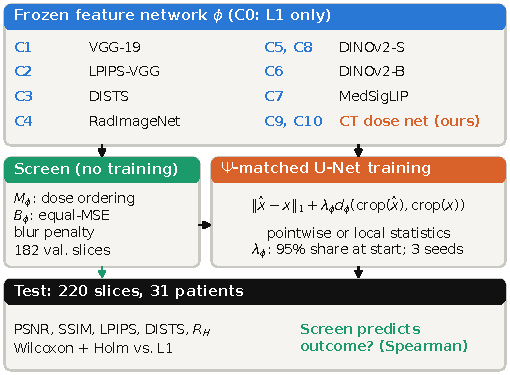
\includegraphics[width=\linewidth]{figures/fig1_overview_column}
  \caption{Only the feature network in the loss changes; its weight is matched by influence, and a screen scores
    each network before training.}
  \label{fig:overview}
\end{figure}
